% =============================================================================
%  Diplomado en Data Science Aplicada con Python para la Toma de Decisiones
%  Clase 1: Fundamentos de Python + Control de Flujo
%  SLB Ecuador | UDLA
%
%  Compilar: pdflatex -shell-escape presentacion.tex (x2 para refs)
% =============================================================================
\documentclass[aspectratio=169, 11pt]{beamer}

% ── Codificación y lenguaje ──────────────────────────────────────────────────
\usepackage[T1]{fontenc}
\usepackage[utf8]{inputenc}
\usepackage[spanish]{babel}

% ── Fuentes ──────────────────────────────────────────────────────────────────
\usepackage{FiraSans}
\usepackage{FiraMono}
\renewcommand{\familydefault}{\sfdefault}

% ── Gráficos y diagramas ────────────────────────────────────────────────────
\usepackage{graphicx}
\usepackage{tikz}
\usetikzlibrary{arrows.meta, positioning, shapes.geometric, calc, fit}
\usepackage{fontawesome5}

% ── Código fuente ────────────────────────────────────────────────────────────
\usepackage{minted}
\usepackage{tcolorbox}
\tcbuselibrary{minted, skins, breakable}

% ── Tablas y utilidades ──────────────────────────────────────────────────────
\usepackage{booktabs}
\usepackage{multicol}
\usepackage{hyperref}
\usepackage{calc}

% =============================================================================
%  PALETA DE COLORES (rojo UDLA + variantes)
% =============================================================================
\definecolor{arcaRed}{HTML}{C82B40}
\definecolor{arcaDark}{HTML}{6B1525}
\definecolor{udlaCrimson}{HTML}{A31545}
\definecolor{arcaGray}{HTML}{F5F5F5}
\definecolor{arcaLightGray}{HTML}{EBEBEB}
\definecolor{textDark}{HTML}{2D2D2D}
\definecolor{textMuted}{HTML}{6B7280}
\definecolor{codeGreen}{HTML}{16A34A}
\definecolor{codeBlue}{HTML}{2563EB}
\definecolor{codeOrange}{HTML}{EA580C}
\definecolor{slbBlue}{HTML}{0014DC}
\definecolor{terminalBg}{HTML}{0F172A}
\definecolor{terminalGreen}{HTML}{86EFAC}
\definecolor{terminalMuted}{HTML}{94A3B8}
\definecolor{codeBg}{HTML}{FAFAFA}

% =============================================================================
%  CONFIGURACIÓN DEL TEMA BEAMER
% =============================================================================
\usetheme{default}
\usecolortheme{default}

% Quitar elementos de navegación por defecto
\setbeamertemplate{navigation symbols}{}
\setbeamertemplate{footline}{}
\setbeamertemplate{headline}{}

% ── Colores de elementos Beamer ──────────────────────────────────────────────
\setbeamercolor{normal text}{fg=textDark}
\setbeamercolor{frametitle}{fg=arcaRed, bg=white}
\setbeamercolor{title}{fg=white}
\setbeamercolor{subtitle}{fg=white!85}
\setbeamercolor{author}{fg=white!80}
\setbeamercolor{date}{fg=white!70}
\setbeamercolor{item}{fg=arcaRed}
\setbeamercolor{subitem}{fg=arcaDark}
\setbeamercolor{block title}{fg=white, bg=arcaRed}
\setbeamercolor{block body}{fg=textDark, bg=arcaGray}
\setbeamercolor{block title alerted}{fg=white, bg=codeOrange}
\setbeamercolor{block body alerted}{fg=textDark, bg=arcaGray}
\setbeamercolor{block title example}{fg=white, bg=codeGreen}
\setbeamercolor{block body example}{fg=textDark, bg=arcaGray}
\setbeamercolor{section in toc}{fg=arcaDark}

% ── Fuentes Beamer ──────────────────────────────────────────────────────────
\setbeamerfont{frametitle}{size=\Large, series=\bfseries}
\setbeamerfont{title}{size=\huge, series=\bfseries}
\setbeamerfont{subtitle}{size=\large}
\setbeamerfont{author}{size=\normalsize}
\setbeamerfont{date}{size=\small}
\setbeamerfont{block title}{size=\normalsize, series=\bfseries}
\setbeamerfont{footnote}{size=\tiny}

% ── Itemize personalizado ───────────────────────────────────────────────────
\setbeamertemplate{itemize item}{\scriptsize\raise1.5pt\hbox{\color{arcaRed}$\blacktriangleright$}}
\setbeamertemplate{itemize subitem}{\scriptsize\raise1pt\hbox{\color{arcaDark}$\bullet$}}
\setbeamertemplate{enumerate items}[default]
\setbeamercolor{enumerate item}{fg=arcaRed}

% =============================================================================
%  HEADER: barra + logos
% =============================================================================
\setbeamertemplate{headline}{%
  \begin{tikzpicture}[remember picture, overlay]
    % Barra superior arcaDark
    \fill[arcaDark] (current page.north west) rectangle
      ([yshift=-0.7cm]current page.north east);
    % Logo UDLA blanco (izquierda)
    \node[anchor=west, inner sep=0pt] at
      ([xshift=0.6cm, yshift=-0.35cm]current page.north west)
      {
\includegraphics[height=0.45cm]{../logo_udla_white.png}};
    % Logo SLB blanco (derecha)
    \node[anchor=east, inner sep=0pt] at
      ([xshift=-0.6cm, yshift=-0.35cm]current page.north east)
      {
\includegraphics[height=0.42cm]{../SLB_white.png}};
  \end{tikzpicture}%
  \vspace{0.7cm}%
}

% =============================================================================
%  FOOTER: número de frame + título corto
% =============================================================================
\setbeamertemplate{footline}{%
  \begin{tikzpicture}[remember picture, overlay]
    % Línea fina
    \draw[arcaLightGray, line width=0.4pt]
      ([yshift=0.55cm, xshift=0.6cm]current page.south west) --
      ([yshift=0.55cm, xshift=-0.6cm]current page.south east);
    % Texto central
    \node[anchor=south, font=\tiny\color{textMuted}] at
      ([yshift=0.15cm]current page.south)
      {Diplomado en Data Science Aplicada con Python \(\cdot\) SLB Ecuador};
    % Número de frame
    \node[anchor=south east, font=\scriptsize\bfseries\color{arcaRed}] at
      ([xshift=-0.6cm, yshift=0.15cm]current page.south east)
      {\insertframenumber};
  \end{tikzpicture}%
}

% =============================================================================
%  FRAMETITLE personalizado con línea roja
% =============================================================================
\setbeamertemplate{frametitle}{%
  \vspace{0.25cm}%
  \usebeamerfont{frametitle}\usebeamercolor[fg]{frametitle}\insertframetitle%
  \par\vspace{2pt}%
  \begin{tikzpicture}
    \fill[arcaRed] (0,0) rectangle (3cm, 1.5pt);
    \fill[arcaLightGray] (3cm,0) rectangle (\textwidth, 0.5pt);
  \end{tikzpicture}%
  \vspace{0.1cm}%
}

% =============================================================================
%  ESTILO DE BLOQUES DE CÓDIGO (minted + tcolorbox)
% =============================================================================
\newtcblisting{pyblock}[1][]{%
  listing engine=minted,
  minted language=python,
  minted style=xcode,
  minted options={
    fontsize=\small,
    linenos=false,
    breaklines=true,
    python3=true
  },
  enhanced,
  colback=codeBg,
  colframe=arcaRed,
  left=8pt,
  right=6pt,
  top=5pt,
  bottom=5pt,
  boxrule=0pt,
  leftrule=3pt,
  arc=3pt,
  listing only,
  title={\hspace{-2pt}\faPython\hspace{5pt}Python},
  fonttitle=\scriptsize\bfseries,
  colbacktitle=arcaRed,
  coltitle=white,
  attach boxed title to top left={xshift=8pt, yshift=-7pt},
  boxed title style={
    arc=2pt, boxrule=0pt,
    top=1.5pt, bottom=1.5pt, left=6pt, right=6pt
  },
  drop fuzzy shadow=black!12,
  #1
}

\newtcblisting{pyblocknum}[1][]{%
  listing engine=minted,
  minted language=python,
  minted style=xcode,
  minted options={
    fontsize=\small,
    linenos=true,
    numbersep=8pt,
    breaklines=true,
    python3=true
  },
  enhanced,
  colback=codeBg,
  colframe=arcaRed,
  left=10pt, right=6pt, top=5pt, bottom=5pt,
  boxrule=0pt,
  leftrule=3pt,
  arc=3pt,
  listing only,
  title={\hspace{-2pt}\faPython\hspace{5pt}Python},
  fonttitle=\scriptsize\bfseries,
  colbacktitle=arcaRed,
  coltitle=white,
  attach boxed title to top left={xshift=8pt, yshift=-7pt},
  boxed title style={
    arc=2pt, boxrule=0pt,
    top=1.5pt, bottom=1.5pt, left=6pt, right=6pt
  },
  #1
}

\newtcblisting{outputblock}[1][]{%
  listing engine=minted,
  minted language=text,
  minted style=bw,
  minted options={
    fontsize=\small,
    breaklines=true,
    formatcom=\color{terminalGreen}
  },
  enhanced,
  colback=terminalBg,
  colframe=terminalBg,
  coltext=terminalGreen,
  left=10pt, right=6pt, top=5pt, bottom=5pt,
  boxrule=0pt,
  arc=3pt,
  listing only,
  title={\hspace{-2pt}\faTerminal\hspace{5pt}Output},
  fonttitle=\scriptsize\bfseries,
  colbacktitle=terminalGreen!85!black,
  coltitle=terminalBg,
  attach boxed title to top left={xshift=8pt, yshift=-7pt},
  boxed title style={
    arc=2pt, boxrule=0pt,
    top=1.5pt, bottom=1.5pt, left=6pt, right=6pt
  },
  #1
}

% =============================================================================
%  COMANDO PARA SECTION DIVIDERS
% =============================================================================
\newcommand{\sectionframe}[2]{%
  \begingroup
    \setbeamertemplate{headline}{}
    \setbeamertemplate{footline}{}
    \setbeamertemplate{navigation symbols}{}
    \begin{frame}[plain, noframenumbering]
      \begin{tikzpicture}[remember picture, overlay]
        \fill[arcaRed] (current page.south west) rectangle (current page.north east);
        \node[anchor=center, text=white, font=\Huge\bfseries, text width=12cm,
              align=center] at ([yshift=0.5cm]current page.center) {#1};
        \node[anchor=center, text=white!80, font=\large, text width=10cm,
              align=center] at ([yshift=-0.8cm]current page.center) {#2};
      \end{tikzpicture}
    \end{frame}
  \endgroup
}

% =============================================================================
%  METADATOS
% =============================================================================
\title{Diplomado en Data Science Aplicada\\con Python para la Toma de Decisiones}
\subtitle{Clase 1: Fundamentos de Python + Control de Flujo}
\author{Carlos Enrique Mosquera Trujillo}
\date{2026}

% =============================================================================
%  DOCUMENTO
% =============================================================================
\begin{document}

% ─────────────────────────────────────────────────────────────────────────────
%  FRAME 1: PORTADA
% ─────────────────────────────────────────────────────────────────────────────
{
\setbeamertemplate{headline}{}
\setbeamertemplate{footline}{}
\begin{frame}[plain, noframenumbering]
  \begin{tikzpicture}[remember picture, overlay]
    % Fondo blanco
    \fill[white] (current page.south west) rectangle (current page.north east);

    % Franja superior arcaRed
    \fill[arcaRed]
      (current page.north west) rectangle
      ([yshift=-0.35cm]current page.north east);

    % Franja inferior arcaDark
    \fill[arcaDark]
      (current page.south west) rectangle
      ([yshift=0.35cm]current page.south east);

    % Línea decorativa vertical izquierda
    \fill[arcaRed]
      ([xshift=1.1cm, yshift=-0.35cm]current page.north west) rectangle
      ([xshift=1.15cm, yshift=0.35cm]current page.south west);

    % Logo UDLA (superior izquierda)
    \node[anchor=north west, inner sep=0pt] at
      ([xshift=1.8cm, yshift=-1.2cm]current page.north west)
      {
\includegraphics[height=1.6cm]{../logo_udla.png}};

    % Logo SLB (superior derecha)
    \node[anchor=north east, inner sep=0pt] at
      ([xshift=-1.5cm, yshift=-1.2cm]current page.north east)
      {
\includegraphics[height=1.5cm]{../SLB.png}};

    % Título principal
    \node[anchor=center, text=arcaDark, text width=13cm, align=center] at
      ([yshift=0.8cm]current page.center) {
        {\huge\bfseries Diplomado en Data Science Aplicada}\\[6pt]
        {\huge\bfseries con Python para la Toma de Decisiones}
      };

    % Línea separadora arcaRed
    \fill[arcaRed]
      ([yshift=-0.4cm, xshift=-3cm]current page.center) rectangle
      ([yshift=-0.33cm, xshift=3cm]current page.center);

    % Subtítulo
    \node[anchor=center, text=arcaRed, font=\Large] at
      ([yshift=-1.1cm]current page.center) {
        Clase 1: Fundamentos de Python + Control de Flujo
      };

    % Instructor
    \node[anchor=center, text=textMuted, font=\normalsize] at
      ([yshift=-2.2cm]current page.center) {
        {\color{arcaRed}\faUser}\hspace{6pt}Carlos Enrique Mosquera Trujillo
        \hspace{16pt}
        {\color{arcaRed}\faIndustry}\hspace{4pt}SLB Ecuador
      };
  \end{tikzpicture}
\end{frame}
}

% ─────────────────────────────────────────────────────────────────────────────
%  FRAME 2: PRESENTACIÓN DEL INSTRUCTOR
% ─────────────────────────────────────────────────────────────────────────────
\begin{frame}{Instructor}
  \vspace{-2pt}
  \begin{columns}[T]
    \begin{column}{0.22\textwidth}
      \centering
      \begin{tikzpicture}
        \clip[rounded corners=3pt] (0,0) rectangle (2.6,2.6);
        \node[anchor=south west, inner sep=0pt] at (0,0)
          {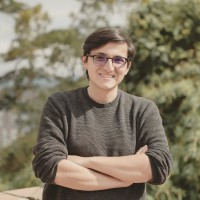
\includegraphics[width=2.6cm]{../Foto Carlos.jpg}};
      \end{tikzpicture}

      \vspace{5pt}
      {\tiny\color{textMuted}
        \faEnvelope\hspace{2pt}\texttt{cmosquerat@unal.edu.co}\\[2pt]
        \faLinkedin\hspace{2pt}cmosquerat56
      }
    \end{column}

    \begin{column}{0.75\textwidth}
      {\normalsize\bfseries\color{arcaDark} Carlos Enrique Mosquera Trujillo}\\[2pt]
      {\footnotesize\color{textMuted} Ingeniero Electrónico \(\cdot\) M.Sc. Automatización Industrial}

      \vspace{6pt}
      {\footnotesize
      \begin{itemize}\setlength{\itemsep}{3pt}
        \item[{\color{arcaRed}\scriptsize\faGraduationCap}] Ing. Electrónica y M.Sc. en Automatización Industrial,
              \textbf{Universidad Nacional de Colombia}.

        \item[{\color{arcaRed}\scriptsize\faPython}] \textbf{6+ años en Python y SQL}:
              pipelines de datos, automatización de reportes, analítica operativa.

        \item[{\color{arcaRed}\scriptsize\faServer}] \textbf{Gestor de HPC} (BIOS):
              cómputo de alto rendimiento para cargas intensivas en datos. Administración de sistemas Linux.

        \item[{\color{arcaRed}\scriptsize\faChalkboardTeacher}] \textbf{Profesor UDLA}:
              Dos años de experiencia en diplomados. PySpark y Metaprogramación.
      \end{itemize}
      }
    \end{column}
  \end{columns}
\end{frame}

% ─────────────────────────────────────────────────────────────────────────────
%  FRAME 3: METODOLOGÍA — PROJECT-BASED LEARNING
% ─────────────────────────────────────────────────────────────────────────────
\begin{frame}{Metodología: Project-Based Learning}
  \vspace{-6pt}
  \begin{columns}[T]
    \begin{column}{0.52\textwidth}
      \centering
      \begin{tikzpicture}[
        node distance=1.1cm,
        stage/.style={
          rectangle, rounded corners=4pt,
          minimum width=3.6cm, minimum height=0.7cm,
          text=white, font=\scriptsize\bfseries,
          align=center
        },
        arrow/.style={
          -{Stealth[length=4pt]}, line width=0.8pt, arcaRed
        },
        label/.style={
          font=\tiny\color{textMuted}, align=right, text width=2.5cm, anchor=east
        }
      ]
        % Nodos del ciclo
        \node[stage, fill=arcaDark]
          (problema) {\faIndustry\hspace{4pt}Problema Real};
        \node[stage, fill=arcaRed, below=0.5cm of problema]
          (concepto) {\faLightbulb\hspace{4pt}Conceptos Clave};
        \node[stage, fill=arcaRed!80!black, below=0.5cm of concepto]
          (codigo) {\faCode\hspace{4pt}Código};
        \node[stage, fill=udlaCrimson, below=0.5cm of codigo]
          (solucion) {\faChartBar\hspace{4pt}Solución};
        \node[stage, fill=arcaDark!80, below=0.5cm of solucion]
          (reflexion) {\faSync\hspace{4pt}Reflexión};

        % Flechas descendentes
        \draw[arrow] (problema) -- (concepto);
        \draw[arrow] (concepto) -- (codigo);
        \draw[arrow] (codigo)   -- (solucion);
        \draw[arrow] (solucion) -- (reflexion);

        % Flecha de retorno (ciclo)
        \draw[arrow, arcaDark!50]
          (reflexion.east) -- ++(0.5,0) |- (problema.east);

        % Etiquetas laterales
        \node[label] at ([xshift=-0.25cm]problema.west)
          {Contexto operativo\\SLB Ecuador};
        \node[label] at ([xshift=-0.25cm]concepto.west)
          {Teoría mínima\\necesaria};
        \node[label] at ([xshift=-0.25cm]codigo.west)
          {Google Colab\\en vivo};
        \node[label] at ([xshift=-0.25cm]solucion.west)
          {Resultado medible\\y auditable};
        \node[label] at ([xshift=-0.25cm]reflexion.west)
          {Siguiente\\iteración};
      \end{tikzpicture}
    \end{column}

    \begin{column}{0.45\textwidth}
      {\small\color{arcaDark}\bfseries Cada sesión de 2h sigue este ciclo:}

      \vspace{6pt}
      {\footnotesize
      \begin{enumerate}\setlength{\itemsep}{3pt}
        \item[\textbf{\color{arcaRed}1.}] Se presenta un \textbf{problema operativo real} de un campo petrolero.

        \item[\textbf{\color{arcaRed}2.}] Se introducen los \textbf{conceptos} necesarios para resolverlo.

        \item[\textbf{\color{arcaRed}3.}] Se escribe \textbf{código en vivo} en Google Colab, juntos.

        \item[\textbf{\color{arcaRed}4.}] Se llega a una \textbf{solución funcional}: un reporte, una métrica.

        \item[\textbf{\color{arcaRed}5.}] Se \textbf{reflexiona}: ¿qué más se podría hacer? Eso motiva la siguiente clase.
      \end{enumerate}
      }


    \end{column}
  \end{columns}
\end{frame}

% ─────────────────────────────────────────────────────────────────────────────
%  FRAME 4: ¿POR QUÉ APRENDER A PROGRAMAR HOY?
% ─────────────────────────────────────────────────────────────────────────────
\begin{frame}{¿Por Qué Aprender a Programar Hoy?}
  \vspace{-4pt}
  {\footnotesize
  \begin{columns}[T]
    \begin{column}{0.48\textwidth}
      {\small\color{arcaDark}\bfseries La IA ya genera código y reportes.}

      \vspace{6pt}
      \begin{itemize}\setlength{\itemsep}{6pt}
        \item[{\color{arcaRed}\scriptsize\faRobot}]
          ChatGPT, Copilot y Claude \textbf{escriben Python}, generan análisis
          y producen reportes completos en segundos.

        \item[{\color{arcaRed}\scriptsize\faExclamationTriangle}]
          Pero \textbf{cometen errores}: calculan mal un corte de agua,
          confunden un pozo con otro, inventan datos que no existen.

        \item[{\color{arcaRed}\scriptsize\faUserShield}]
          Quien \textbf{sabe leer código} detecta el error antes de
          que llegue a una decisión operativa.
          Quien no, lo publica como verdad.
      \end{itemize}
    \end{column}

    \begin{column}{0.48\textwidth}
      {\small\color{arcaDark}\bfseries Programar no es competir con la IA.\\
      Es saber dirigirla.}

      \vspace{6pt}
      \begin{itemize}\setlength{\itemsep}{6pt}
        \item[{\color{arcaRed}\scriptsize\faSearch}]
          \textbf{Auditar}: leer el código que la IA genera y
          verificar que la lógica sea correcta.

        \item[{\color{arcaRed}\scriptsize\faSlidersH}]
          \textbf{Ajustar}: modificar parámetros, corregir fórmulas,
          adaptar la solución al contexto real.

        \item[{\color{arcaRed}\scriptsize\faProjectDiagram}]
          \textbf{Orquestar}: conectar múltiples herramientas
          de IA en un flujo de trabajo confiable.
      \end{itemize}

      \vspace{6pt}
      {\scriptsize\color{textMuted}\itshape
        Este diplomado nos prepara para ese rol:
        el profesional que entiende, valida y decide.}
    \end{column}
  \end{columns}
  }
\end{frame}

% ─────────────────────────────────────────────────────────────────────────────
%  FRAME 5: HUMAN-IN-THE-LOOP
% ─────────────────────────────────────────────────────────────────────────────
\begin{frame}{Human-in-the-Loop}
  \vspace{-2pt}
  \centering
  \begin{tikzpicture}[
    box/.style={
      rectangle, rounded corners=5pt,
      minimum width=3.4cm, minimum height=1cm,
      font=\small\bfseries, align=center,
      text=white
    },
    arrow/.style={
      -{Stealth[length=6pt]}, line width=1.4pt, arcaRed
    },
    lbl/.style={
      font=\scriptsize\color{textMuted}, fill=white, inner sep=2pt
    },
    node distance=1.6cm and 3.8cm
  ]
    % ── Fila superior ──
    \node[box, fill=arcaDark]
      (instruccion) {\faKeyboard\hspace{4pt}Instrucción};
    \node[box, fill=arcaRed, right=of instruccion]
      (agente) {\faRobot\hspace{4pt}Agente IA};

    % ── Fila inferior ──
    \node[box, fill=udlaCrimson, below=of agente]
      (output) {\faFile\hspace{4pt}Output};
    \node[box, fill=arcaDark!85, below=of instruccion]
      (valida) {\faUserCheck\hspace{4pt}Validación Humana};

    % ── Ciclo clockwise ──
    \draw[arrow] (instruccion) -- (agente)
      node[lbl, midway, above] {envía prompt};
    \draw[arrow] (agente) -- (output)
      node[lbl, midway, right] {genera código};
    \draw[arrow] (output) -- (valida)
      node[lbl, midway, below] {revisa resultado};
    \draw[arrow, arcaDark!70] (valida) -- (instruccion)
      node[lbl, midway, left] {ajusta};

    % ── Decisión: aprueba ──
    \node[box, fill=codeGreen, minimum width=2.8cm, minimum height=0.8cm,
          below=1.2cm of valida]
      (aprueba) {\faCheck\hspace{3pt}A Producción};

    \draw[-{Stealth[length=5pt]}, line width=1.2pt, codeGreen!80!black]
      (valida) -- (aprueba)
      node[lbl, midway, right] {correcto};

  \end{tikzpicture}

  \vspace{8pt}

\end{frame}

% ─────────────────────────────────────────────────────────────────────────────
%  FRAME 6: ¿POR QUÉ PYTHON?
% ─────────────────────────────────────────────────────────────────────────────
\begin{frame}{¿Por Qué Python?}
  \vspace{-2pt}
  \centering

  {\small\color{arcaDark}\bfseries
    \#1 en TIOBE, Stack Overflow y GitHub desde 2021.}

  \vspace{10pt}
  \begin{columns}[T]
    \begin{column}{0.22\textwidth}
      \centering
      {\Huge\color{arcaRed}\faChartLine}\\[6pt]
      {\small\bfseries\color{arcaDark} Legible}\\[3pt]
      {\scriptsize\color{textMuted} Sintaxis clara: se lee\\
      casi como inglés técnico.\\
      Menos código, menos errores.}
    \end{column}

    \begin{column}{0.22\textwidth}
      \centering
      {\Huge\color{arcaRed}\faCubes}\\[6pt]
      {\small\bfseries\color{arcaDark} Ecosistema}\\[3pt]
      {\scriptsize\color{textMuted} \texttt{pandas}, \texttt{numpy},\\
      \texttt{lasio}, \texttt{scikit-learn}.\\
      Todo resuelto y documentado.}
    \end{column}

    \begin{column}{0.22\textwidth}
      \centering
      {\Huge\color{arcaRed}\faIndustry}\\[6pt]
      {\small\bfseries\color{arcaDark} Industrial}\\[3pt]
      {\scriptsize\color{textMuted} SLB, Shell, Chevron,\\
      ExxonMobil, Petrobras, NASA.\\
      Petrofísica, producción, forecasting.}
    \end{column}

    \begin{column}{0.22\textwidth}
      \centering
      {\Huge\color{arcaRed}\faGraduationCap}\\[6pt]
      {\small\bfseries\color{arcaDark} Académico}\\[3pt]
      {\scriptsize\color{textMuted} Lenguaje de referencia en\\
      MIT, Stanford y Harvard\\
      para cursos introductorios.}
    \end{column}
  \end{columns}

  \vspace{12pt}
  {\footnotesize\color{arcaDark}\itshape
    Python no es un lenguaje académico. Es infraestructura de negocio.}
\end{frame}

% ─────────────────────────────────────────────────────────────────────────────
%  FRAME 7: PYTHON EN LA OPERACIÓN
% ─────────────────────────────────────────────────────────────────────────────
\begin{frame}{Python en la Operación Diaria}
  \vspace{-2pt}
  {\small\color{arcaDark}\bfseries
    Con este diplomado vamos a automatizar tareas como estas:}

  \vspace{10pt}
  \begin{columns}[T]
    \begin{column}{0.30\textwidth}
      \centering
      {\Huge\color{arcaRed}\faFileExcel}\\[8pt]
      {\small\bfseries\color{arcaDark} Reportes}\\[4pt]
      {\scriptsize\color{textMuted}
        Leer 50 archivos LAS de\\
        well logs, consolidar en\\
        un dataset y exportar KPIs.\\[4pt]
        \textbf{4 horas manual} $\rightarrow$ \textbf{30 seg}}
    \end{column}

    \begin{column}{0.30\textwidth}
      \centering
      {\Huge\color{arcaRed}\faChartBar}\\[8pt]
      {\small\bfseries\color{arcaDark} Análisis}\\[4pt]
      {\scriptsize\color{textMuted}
        Cruzar producción diaria con\\
        registros de sensores,\\
        detectar caídas de flujo.\\[4pt]
        \textbf{Sin depender de TI}}
    \end{column}

    \begin{column}{0.30\textwidth}
      \centering
      {\Huge\color{arcaRed}\faRobot}\\[8pt]
      {\small\bfseries\color{arcaDark} IA Aplicada}\\[4pt]
      {\scriptsize\color{textMuted}
        Predecir producción por pozo,\\
        clasificar litologías y\\
        optimizar intervenciones.\\[4pt]
        \textbf{Objetivo del diplomado}}
    \end{column}
  \end{columns}

  \vspace{14pt}
  \centering
  {\footnotesize\color{arcaDark}
    \textbf{No necesitamos ser programadores.}
    Necesitamos saber lo suficiente para dirigir, auditar y decidir.}
\end{frame}

% ─────────────────────────────────────────────────────────────────────────────
%  SECTION DIVIDER: ENTORNO DE TRABAJO
% ─────────────────────────────────────────────────────────────────────────────
\sectionframe{Entorno de Trabajo}{Google Colab y repositorio del curso}

% ─────────────────────────────────────────────────────────────────────────────
%  FRAME 8: ¿QUÉ ES GOOGLE COLAB?
% ─────────────────────────────────────────────────────────────────────────────
\begin{frame}{¿Qué es Google Colab?}
  \vspace{-6pt}
  \begin{columns}[T]
    \begin{column}{0.52\textwidth}
      {\small\color{arcaDark}\bfseries
        Entorno de programación en la nube. Gratuito. Cero instalaciones.}

      \vspace{6pt}
      {\footnotesize
      \begin{itemize}\setlength{\itemsep}{4pt}
        \item[{\color{arcaRed}\scriptsize\faCloud}]
          Solo necesitamos una cuenta de Google y un navegador.

        \item[{\color{arcaRed}\scriptsize\faPuzzlePiece}]
          Organizado en \textbf{celdas}: código $\rightarrow$ ejecución $\rightarrow$ resultado.

        \item[{\color{arcaRed}\scriptsize\faUsers}]
          Se comparte como un Google Doc. Trabajo colaborativo.

        \item[{\color{arcaRed}\scriptsize\faServer}]
          Google provee CPU, RAM y GPU sin costo.
      \end{itemize}
      }
    \end{column}

    \begin{column}{0.43\textwidth}
      \centering
      \vspace{2pt}
      \begin{tikzpicture}[
        box/.style={rectangle, rounded corners=3pt, draw=arcaLightGray,
          fill=arcaGray, minimum width=3.8cm, minimum height=0.55cm,
          font=\scriptsize, align=left, text=textDark},
        node distance=0.2cm
      ]
        \node[box] (c1) {\texttt{\color{codeBlue}{pozo} = \color{codeGreen}{'Sacha042'}}};
        \node[box, below=of c1] (c2) {\texttt{\color{codeBlue}{bopd} = \color{codeOrange}{1250}}};
        \node[box, below=of c2, fill=white, draw=arcaLightGray]
          (o1) {\texttt{> Sacha042}};
        \node[box, below=of o1] (c3) {\texttt{\color{codeBlue}{print}(pozo)}};
        \node[box, below=of c3, fill=white, draw=arcaLightGray]
          (o2) {\texttt{> 1250}};

        \node[font=\tiny\color{textMuted}, left=0.1cm of c1] {[\,1\,]};
        \node[font=\tiny\color{textMuted}, left=0.1cm of c2] {[\,2\,]};
        \node[font=\tiny\color{textMuted}, left=0.1cm of c3] {[\,3\,]};
      \end{tikzpicture}
    \end{column}
  \end{columns}
\end{frame}

% ─────────────────────────────────────────────────────────────────────────────
%  FRAME 9: REPOSITORIO DEL CURSO
% ─────────────────────────────────────────────────────────────────────────────
\begin{frame}{Repositorio del Curso}
  \vspace{-6pt}
  \begin{columns}[T]
    \begin{column}{0.52\textwidth}
      {\small\color{arcaDark}\bfseries
        Todo el material centralizado. Un link, todo el curso.}

      \vspace{4pt}
      {\footnotesize
      \begin{itemize}\setlength{\itemsep}{3pt}
        \item[{\color{arcaRed}\scriptsize\faFolderOpen}]
          \textbf{Presentaciones}: slides de cada clase en PDF.

        \item[{\color{arcaRed}\scriptsize\faLaptopCode}]
          \textbf{Notebooks}: cuadernos Colab con ejercicios y micro-proyectos.

        \item[{\color{arcaRed}\scriptsize\faDatabase}]
          \textbf{Datos}: datasets petroleros para las prácticas.

        \item[{\color{arcaRed}\scriptsize\faCodeBranch}]
          \textbf{Versionado}: cada clase se publica como nueva versión.
      \end{itemize}
      }

      \vspace{4pt}
      \begin{tcolorbox}[
        colback=arcaGray, colframe=arcaRed, boxrule=0pt, leftrule=3pt,
        arc=2pt, left=5pt, right=5pt, top=3pt, bottom=3pt
      ]
        {\scriptsize\color{arcaRed}\faGithub\hspace{4pt}\bfseries Repositorio:}\\[1pt]
        {\scriptsize\ttfamily\color{textDark} github.com/cmosquerat/slb-diplomado}
      \end{tcolorbox}
    \end{column}

    \begin{column}{0.43\textwidth}
      \centering
      \vspace{2pt}
      \begin{tikzpicture}[
        folder/.style={rectangle, rounded corners=3pt,
          minimum width=3.8cm, minimum height=0.5cm,
          font=\scriptsize\ttfamily, align=left, text=textDark,
          fill=arcaGray, draw=arcaLightGray},
        node distance=0.2cm
      ]
        \node[folder, fill=arcaDark, text=white, font=\scriptsize\ttfamily\bfseries]
          (root) {slb-diplomado/};
        \node[folder, below=of root]  (c01) {~~clase-01/};
        \node[folder, below=of c01]   (c02) {~~clase-02/};
        \node[folder, below=of c02]   (dots) {~~clase-03/};
        \node[folder, below=of dots]  (data) {~~datos/};
        \node[folder, below=of data]  (readme) {~~README.md};
      \end{tikzpicture}
    \end{column}
  \end{columns}
\end{frame}

% ─────────────────────────────────────────────────────────────────────────────
%  FRAME 10: CÓMO ABRIR GOOGLE COLAB
% ─────────────────────────────────────────────────────────────────────────────
\begin{frame}{Abrir Google Colab}
  \vspace{-6pt}
  \centering
  \begin{tikzpicture}[
    sbox/.style={rectangle, rounded corners=5pt, fill=arcaGray,
      draw=arcaLightGray, minimum width=2.8cm, minimum height=1.7cm,
      font=\scriptsize, align=center, text=textDark},
    snum/.style={circle, fill=arcaRed, text=white, font=\small\bfseries,
      minimum size=0.55cm, inner sep=0pt},
    sarrow/.style={-{Stealth[length=5pt]}, line width=1.2pt, arcaRed},
    node distance=0.8cm
  ]
    \node[sbox] (s1) {{\Large\color{arcaRed}\faGoogle}\\[4pt]Ir a\\[1pt]\texttt{\bfseries colab.google.com}};
    \node[sbox, right=of s1] (s2) {{\Large\color{arcaRed}\faKey}\\[4pt]Iniciar sesión con\\[1pt]su \textbf{cuenta Google}};
    \node[sbox, right=of s2] (s3) {{\Large\color{arcaRed}\faPlus}\\[4pt]Click en\\[1pt]\textbf{Nuevo cuaderno}};
    \node[sbox, right=of s3] (s4) {{\Large\color{arcaRed}\faPlay}\\[4pt]Escribir código\\[1pt]y presionar \textbf{Play}};

    \node[snum, above=0.15cm of s1] {1};
    \node[snum, above=0.15cm of s2] {2};
    \node[snum, above=0.15cm of s3] {3};
    \node[snum, above=0.15cm of s4] {4};

    \draw[sarrow] (s1) -- (s2);
    \draw[sarrow] (s2) -- (s3);
    \draw[sarrow] (s3) -- (s4);
  \end{tikzpicture}

  \vspace{10pt}
  {\footnotesize\color{arcaDark}
    \textbf{Hagámoslo ahora.} Abramos \texttt{colab.google.com} y creemos un cuaderno nuevo.}
\end{frame}

% ─────────────────────────────────────────────────────────────────────────────
%  SECTION DIVIDER: FUNDAMENTOS
% ─────────────────────────────────────────────────────────────────────────────
\sectionframe{Fundamentos de Python}{Antes de escribir código}

% ─────────────────────────────────────────────────────────────────────────────
%  FRAME 11: ¿QUÉ ES PROGRAMAR?
% ─────────────────────────────────────────────────────────────────────────────
\begin{frame}{¿Qué es Programar?}
  \vspace{-6pt}
  {\small\color{arcaDark}\bfseries
    Descomponer un problema en pasos que una máquina pueda ejecutar.}

  \vspace{4pt}
  \begin{columns}[T]
    \begin{column}{0.38\textwidth}
      \begin{tcolorbox}[
        colback=arcaDark, colframe=arcaDark, boxrule=0pt,
        arc=4pt, left=6pt, right=6pt, top=5pt, bottom=5pt
      ]
        {\scriptsize\color{white}\bfseries\faIndustry\hspace{4pt}Problema operativo}\\[3pt]
        {\scriptsize\color{white!85}\itshape
        ``¿Cuál es la utilidad neta\\
        del pozo Sacha-042 hoy?''}
      \end{tcolorbox}

      \vspace{4pt}
      {\scriptsize\color{textMuted}
        Una computadora no interpreta esta frase.
        No sabe qué es ``utilidad'', ni dónde están los datos.
        \textbf{Necesitamos descomponerlo en pasos.}}
    \end{column}

    \begin{column}{0.06\textwidth}
      \centering
      \vspace{20pt}
      {\Large\color{arcaRed}$\Rightarrow$}
    \end{column}

    \begin{column}{0.50\textwidth}
      \begin{tcolorbox}[
        colback=arcaGray, colframe=arcaRed, boxrule=0pt, leftrule=3pt,
        arc=3pt, left=5pt, right=5pt, top=4pt, bottom=4pt
      ]
        {\scriptsize\color{arcaRed}\bfseries Paso 1:} {\scriptsize Definir producción (BOPD)}\\
        {\scriptsize\ttfamily\color{textDark} bopd = 1250}\\[3pt]
        {\scriptsize\color{arcaRed}\bfseries Paso 2:} {\scriptsize Definir precio del crudo}\\
        {\scriptsize\ttfamily\color{textDark} precio = 72.50}\\[3pt]
        {\scriptsize\color{arcaRed}\bfseries Paso 3:} {\scriptsize Definir costo por barril}\\
        {\scriptsize\ttfamily\color{textDark} costo = 38.00}\\[3pt]
        {\scriptsize\color{arcaRed}\bfseries Paso 4:} {\scriptsize Calcular y mostrar utilidad}\\
        {\scriptsize\ttfamily\color{textDark} print(bopd * (precio - costo))}
      \end{tcolorbox}
    \end{column}
  \end{columns}

  \vspace{4pt}
  {\footnotesize\color{arcaDark}
    \textbf{Programar = pensar con precisión.}
    El mismo proceso que ya hacemos en una hoja de cálculo, pero sin ambigüedad.}
\end{frame}

% ─────────────────────────────────────────────────────────────────────────────
%  FRAME 12: SINTAXIS
% ─────────────────────────────────────────────────────────────────────────────
\begin{frame}[fragile]{Sintaxis: La Gramática de Python}
  \vspace{-6pt}
  \begin{columns}[T]
    \begin{column}{0.48\textwidth}
      {\small\color{arcaDark}\bfseries
        Así como el español tiene reglas,
        Python tiene \textbf{sintaxis}.}

      \vspace{4pt}
      {\footnotesize\color{textMuted}
      \begin{itemize}\setlength{\itemsep}{3pt}
        \item[{\color{arcaRed}\scriptsize\faFont}]
          \textbf{Mayúsculas importan}: \texttt{print} no es \texttt{Print}.

        \item[{\color{arcaRed}\scriptsize\faCode}]
          \textbf{Paréntesis obligatorios}: toda función
          lleva \texttt{()}.

        \item[{\color{arcaRed}\scriptsize\faQuoteRight}]
          \textbf{Comillas para texto}: \texttt{"hola"} es texto,
          \texttt{hola} sin comillas es una variable.

        \item[{\color{arcaRed}\scriptsize\faIndent}]
          \textbf{Indentación}: los espacios al inicio
          definen la estructura del código.
      \end{itemize}
      }
    \end{column}

    \begin{column}{0.48\textwidth}
      {\small\color{codeGreen}\bfseries\faCheck\hspace{4pt}Correcto}
      \begin{tcolorbox}[
        colback=arcaGray, colframe=codeGreen, boxrule=0pt, leftrule=3pt,
        arc=2pt, left=5pt, right=5pt, top=3pt, bottom=3pt
      ]
        {\scriptsize\ttfamily\color{textDark}
        bopd = 1250\\
        print(bopd)}
      \end{tcolorbox}

      \vspace{3pt}
      {\small\color{arcaRed}\bfseries\faTimes\hspace{4pt}Errores comunes}
      \begin{tcolorbox}[
        colback=arcaGray, colframe=arcaRed, boxrule=0pt, leftrule=3pt,
        arc=2pt, left=5pt, right=5pt, top=2pt, bottom=2pt
      ]
        {\scriptsize\ttfamily\color{textDark}
        Print(bopd)\hspace{10pt}}{\tiny\color{arcaRed} P mayúscula}\\
        {\scriptsize\ttfamily\color{textDark}
        print(bopd\hspace{12pt}}{\tiny\color{arcaRed} falta )}\\
        {\scriptsize\ttfamily\color{textDark}
        print bopd\hspace{12pt}}{\tiny\color{arcaRed} faltan ()}
      \end{tcolorbox}

      \vspace{2pt}
      {\scriptsize\color{textMuted}\itshape
        Un solo carácter mal y Python nos avisa con un error.}
    \end{column}
  \end{columns}
\end{frame}

% ─────────────────────────────────────────────────────────────────────────────
%  FRAME 13: print() + OPERACIONES (COMBINADO)
% ─────────────────────────────────────────────────────────────────────────────
\begin{frame}[fragile,shrink=10]{\texttt{print()} y Operaciones}
  \vspace{-6pt}
  {\small\color{arcaDark}\bfseries
    \texttt{print()} muestra un valor en pantalla. Python también sabe hacer cuentas.}

  \vspace{4pt}
  \begin{columns}[T]
    \begin{column}{0.54\textwidth}
      \begin{pyblock}[title={\scriptsize\faPlay\hspace{4pt}Escribamos esto en Colab}]
print("Hola SLB Ecuador")
print(1250 * 72.50)
print(1250 * (72.50 - 38.00))
print(1250 ** 2)
      \end{pyblock}
      \vspace{-2pt}
      \begin{outputblock}
Hola SLB Ecuador
90625.0
43125.0
1562500
      \end{outputblock}
    \end{column}

    \begin{column}{0.42\textwidth}
      {\footnotesize
      \renewcommand{\arraystretch}{1.25}
      \begin{tabular}{@{}c l@{}}
        \toprule
        {\bfseries\color{arcaRed} Op.} & {\bfseries\color{arcaDark} Significado} \\
        \midrule
        \texttt{+ \ -} & Suma, resta \\
        \texttt{* \ /} & Producto, división \\
        \texttt{**}    & Potencia \\
        \texttt{//}    & División entera \\
        \texttt{\%}    & Residuo (módulo) \\
        \bottomrule
      \end{tabular}
      }

      \vspace{4pt}
      {\scriptsize\color{textMuted}
        Respeta el orden matemático:
        primero \texttt{*} y \texttt{/},
        después \texttt{+} y \texttt{-}.\\[2pt]
        \textbf{Shift + Enter} ejecuta la celda.}
    \end{column}
  \end{columns}
\end{frame}

% ─────────────────────────────────────────────────────────────────────────────
%  FRAME 14: PRÁCTICA GUIADA
% ─────────────────────────────────────────────────────────────────────────────
\begin{frame}[fragile]{Práctica Guiada \hfill {\normalsize\color{arcaRed}\faClock\hspace{4pt}5 min}}
  \vspace{-6pt}
  {\small\color{arcaDark}\bfseries
    El pozo Sacha-042 produce 1\,250 barriles/día (BOPD). El crudo se vende a \$\,72.50/bbl.}

  \vspace{4pt}
  {\footnotesize\color{textMuted}
  Usando solo \texttt{print()} y operaciones, calculemos en Colab:}

  \vspace{3pt}
  {\footnotesize
  \begin{enumerate}\setlength{\itemsep}{2pt}
    \item[{\color{arcaRed}\bfseries 1.}]
      El \textbf{ingreso bruto diario} del pozo.
    \item[{\color{arcaRed}\bfseries 2.}]
      Si el costo operativo es \$\,38.00/bbl, ¿cuál es la \textbf{utilidad diaria}?
    \item[{\color{arcaRed}\bfseries 3.}]
      ¿Cuál es el \textbf{margen operativo} en porcentaje?
  \end{enumerate}
  }

  \vspace{4pt}
  {\footnotesize\color{textMuted}
    \faLightbulb[regular]\hspace{4pt}\textbf{Pista:}
    Margen = (precio $-$ costo) / precio $\times$ 100}

  \vspace{4pt}
  \begin{pyblock}[title={\scriptsize\faPlay\hspace{4pt}Tres print, tres respuestas}]
print( ___ )
print( ___ )
print( ___ )
  \end{pyblock}
\end{frame}

% ─────────────────────────────────────────────────────────────────────────────
%  FRAME 15: SOLUCIÓN — PRÁCTICA GUIADA
% ─────────────────────────────────────────────────────────────────────────────
\begin{frame}[fragile,shrink=10]{Solución --- Práctica Guiada}
  \vspace{-6pt}
  \begin{columns}[T]
    \begin{column}{0.54\textwidth}
      \begin{pyblock}
print(1250 * 72.50)
print(1250 * 72.50 - 1250 * 38.00)
print((72.50 - 38.00) / 72.50 * 100)
      \end{pyblock}
      \vspace{-2pt}
      \begin{outputblock}
90625.0
43125.0
47.586206896551715
      \end{outputblock}
    \end{column}

    \begin{column}{0.42\textwidth}
      {\footnotesize\color{textMuted}
      \begin{itemize}\setlength{\itemsep}{4pt}
        \item[{\color{codeGreen}\scriptsize\faCheck}]
          Ingreso bruto: \$\,90\,625/día.
        \item[{\color{codeGreen}\scriptsize\faCheck}]
          Utilidad diaria: \$\,43\,125.
        \item[{\color{codeGreen}\scriptsize\faCheck}]
          Margen operativo: 47.6\%.
        \item[{\color{arcaRed}\scriptsize\faExclamationTriangle}]
          Escribimos \texttt{1250} y \texttt{72.50}
          \textbf{tres veces}. Si cambian, corregimos
          todo a mano.
      \end{itemize}
      }
    \end{column}
  \end{columns}
\end{frame}

% ─────────────────────────────────────────────────────────────────────────────
%  SECTION: VARIABLES
% ─────────────────────────────────────────────────────────────────────────────
\sectionframe{Variables y Tipos}{Nombres, valores y conversiones}

% ─────────────────────────────────────────────────────────────────────────────
%  FRAME 16: VARIABLES — ASIGNAR Y REUTILIZAR
% ─────────────────────────────────────────────────────────────────────────────
\begin{frame}[fragile,shrink=10]{Variables: Asignar y Reutilizar}
  \vspace{-6pt}
  {\small\color{arcaDark}\bfseries
    Una variable es un nombre que apunta a un valor en memoria.}

  \vspace{3pt}
  \begin{columns}[T]
    \begin{column}{0.52\textwidth}
      \begin{pyblock}
bopd = 1250
precio = 72.50
costo = 38.00
ingreso = bopd * precio
utilidad = ingreso - bopd * costo
print(ingreso)
print(utilidad)
      \end{pyblock}
      \vspace{-2pt}
      \begin{outputblock}
90625.0
43125.0
      \end{outputblock}
    \end{column}

    \begin{column}{0.44\textwidth}
      {\scriptsize\color{textMuted}
      \begin{itemize}\setlength{\itemsep}{3pt}
        \item[{\color{arcaRed}\scriptsize\faArrowRight}]
          \texttt{=} no es ``igual a''.
          Significa \textbf{asignar}: valor de la
          derecha se guarda con el nombre de la izquierda.
        \item[{\color{arcaRed}\scriptsize\faArrowRight}]
          Si el precio del crudo sube a \$\,78, cambiamos
          \textbf{una sola línea} y todo se recalcula.
        \item[{\color{arcaRed}\scriptsize\faExclamationTriangle}]
          \texttt{Precio} $\neq$ \texttt{precio}.
          Python distingue mayúsculas.
      \end{itemize}
      }
    \end{column}
  \end{columns}
\end{frame}

% ─────────────────────────────────────────────────────────────────────────────
%  FRAME 17: NOMBRAR BIEN — CONVENCIONES
% ─────────────────────────────────────────────────────────────────────────────
\begin{frame}[fragile]{Nombrar Bien Importa}
  \vspace{-6pt}
  {\small\color{arcaDark}\bfseries
    Un buen nombre hace que el código se explique solo.}

  \vspace{6pt}
  \begin{columns}[T]
    \begin{column}{0.48\textwidth}
      {\footnotesize
      \renewcommand{\arraystretch}{1.4}
      \begin{tabular}{@{}l l@{}}
        \toprule
        {\color{codeGreen}\bfseries\faCheck\hspace{3pt}Correcto}
        & {\color{arcaRed}\bfseries\faTimes\hspace{3pt}Evitar} \\
        \midrule
        \texttt{bopd\_pozo} & \texttt{b} \\
        \texttt{precio\_crudo} & \texttt{p1} \\
        \texttt{corte\_agua\_pct} & \texttt{dato} \\
        \texttt{costo\_op\_bbl} & \texttt{x} \\
        \bottomrule
      \end{tabular}
      }

      \vspace{6pt}
      {\scriptsize\color{textMuted}
        Convención en Python: \texttt{snake\_case}\\
        palabras en minúscula separadas por \texttt{\_}}
    \end{column}

    \begin{column}{0.48\textwidth}
      {\footnotesize\color{arcaDark}\bfseries Reglas del lenguaje:}

      \vspace{4pt}
      {\footnotesize\color{textMuted}
      \begin{itemize}\setlength{\itemsep}{3pt}
        \item[{\color{codeGreen}\scriptsize\faCheck}]
          Empieza con letra o \texttt{\_}
        \item[{\color{codeGreen}\scriptsize\faCheck}]
          Puede contener letras, números, \texttt{\_}
        \item[{\color{arcaRed}\scriptsize\faTimes}]
          No puede empezar con número
        \item[{\color{arcaRed}\scriptsize\faTimes}]
          No puede tener espacios ni \texttt{-}
        \item[{\color{arcaRed}\scriptsize\faTimes}]
          No usar palabras reservadas:\\
          \texttt{print}, \texttt{if}, \texttt{for}, \texttt{True}\ldots
      \end{itemize}
      }
    \end{column}
  \end{columns}
\end{frame}

% ─────────────────────────────────────────────────────────────────────────────
%  FRAME 18: TIPOS DE DATOS
% ─────────────────────────────────────────────────────────────────────────────
\begin{frame}[fragile]{Tipos de Datos}
  \vspace{-6pt}
  {\small\color{arcaDark}\bfseries
    Python clasifica cada valor. El tipo determina qué operaciones son válidas.}

  \vspace{3pt}
  \begin{center}
  {\footnotesize
  \renewcommand{\arraystretch}{1.3}
  \begin{tabular}{c l l l}
    \toprule
    & {\bfseries\color{arcaDark} Tipo}
    & {\bfseries\color{arcaDark} Ejemplo}
    & {\bfseries\color{arcaDark} Uso en operación} \\
    \midrule
    {\color{arcaRed}\faHashtag}
    & \texttt{int} --- entero
    & \texttt{1250}
    & Barriles, número de pozos \\
    {\color{arcaRed}\faPercent}
    & \texttt{float} --- decimal
    & \texttt{72.50}
    & Precios, cortes de agua, porosidad \\
    {\color{arcaRed}\faFont}
    & \texttt{str} --- texto
    & \texttt{"Sacha-042"}
    & Nombre de pozo, campo, formación \\
    {\color{arcaRed}\faToggleOn}
    & \texttt{bool} --- lógico
    & \texttt{True / False}
    & ¿Pozo activo? ¿Supera cutoff? \\
    \bottomrule
  \end{tabular}
  }
  \end{center}

  \vspace{2pt}
  \begin{pyblock}
print(type(1250))
print(type(72.50))
print(type("Sacha-042"))
print(type(True))
  \end{pyblock}
\end{frame}

% ─────────────────────────────────────────────────────────────────────────────
%  FRAME 19: CUIDADO AL MEZCLAR TIPOS
% ─────────────────────────────────────────────────────────────────────────────
\begin{frame}[fragile,shrink=10]{Cuidado al Mezclar Tipos}
  \vspace{-6pt}
  {\small\color{arcaDark}\bfseries
    Sumar texto con número no funciona. Python nos avisa con un error.}

  \vspace{6pt}
  \begin{columns}[T]
    \begin{column}{0.48\textwidth}
      {\scriptsize\color{arcaRed}\bfseries\faTimes\hspace{4pt}Esto falla}
      \begin{pyblock}
print("BOPD: " + 1250)
      \end{pyblock}
      \vspace{2pt}
      \begin{outputblock}
TypeError: can only concatenate
str to str (not "int")
      \end{outputblock}
    \end{column}

    \begin{column}{0.48\textwidth}
      {\scriptsize\color{codeGreen}\bfseries\faCheck\hspace{4pt}Dos soluciones}
      \begin{pyblock}
print("BOPD: " + str(1250))
print("BOPD:", 1250)
      \end{pyblock}
      \vspace{2pt}
      \begin{outputblock}
BOPD: 1250
BOPD: 1250
      \end{outputblock}
    \end{column}
  \end{columns}

  \vspace{6pt}
  {\footnotesize\color{textMuted}
    \faLightbulb[regular]\hspace{4pt}%
    \texttt{str()}, \texttt{int()} y \texttt{float()} \textbf{convierten} entre tipos.
    Usaremos esto en la siguiente diapositiva con \texttt{input()}.}
\end{frame}

% ─────────────────────────────────────────────────────────────────────────────
%  FRAME 20: input() — DEDICADO Y BIEN EXPLICADO
% ─────────────────────────────────────────────────────────────────────────────
\begin{frame}[fragile,shrink=15]{\texttt{input()} --- Leer Datos del Usuario}
  \vspace{-6pt}
  {\small\color{arcaDark}\bfseries
    \texttt{input()} \textbf{pausa} el programa y espera a que el usuario escriba.}

  \vspace{4pt}
  \centering
  \begin{tikzpicture}[
    box/.style={rectangle, rounded corners=4pt, minimum height=0.75cm,
      font=\scriptsize\bfseries, align=center, text=white,
      minimum width=2.4cm, inner sep=4pt},
    arr/.style={-{Stealth[length=5pt]}, line width=1pt, arcaRed},
    lbl/.style={font=\tiny\color{textMuted}, fill=white, inner sep=1pt}
  ]
    \node[box, fill=arcaDark] (call) {\faKeyboard\hspace{3pt}\texttt{input("Pozo: ")}};
    \node[box, fill=arcaRed, right=0.9cm of call] (pause) {\faPause\hspace{3pt}Pausa};
    \node[box, fill=udlaCrimson, right=0.9cm of pause] (user) {\faUser\hspace{3pt}Sacha-042};
    \node[box, fill=arcaDark!85, right=0.9cm of user] (ret) {\faQuoteRight\hspace{3pt}\texttt{"Sacha-042"}};

    \draw[arr] (call) -- (pause) node[lbl, midway, above] {ejecuta};
    \draw[arr] (pause) -- (user) node[lbl, midway, above] {espera};
    \draw[arr] (user) -- (ret) node[lbl, midway, above] {devuelve \texttt{str}};
  \end{tikzpicture}

  \vspace{6pt}
  \begin{columns}[T]
    \begin{column}{0.48\textwidth}
      \begin{pyblock}
pozo = input("Pozo: ")
print(pozo)
print(type(pozo))
      \end{pyblock}
      \vspace{2pt}
      \begin{outputblock}
Pozo: Sacha-042
Sacha-042
<class 'str'>
      \end{outputblock}
    \end{column}

    \begin{column}{0.48\textwidth}
      {\scriptsize\color{textMuted}
      \begin{itemize}\setlength{\itemsep}{3pt}
        \item[{\color{arcaRed}\scriptsize\faArrowRight}]
          El texto entre paréntesis es el \textbf{mensaje} que ve el usuario.
        \item[{\color{arcaRed}\scriptsize\faArrowRight}]
          Lo que el usuario escribe se guarda en la variable
          (\texttt{pozo}) como \textbf{cadena de texto (\texttt{str})}.
        \item[{\color{arcaRed}\scriptsize\faExclamationTriangle}]
          Aunque el usuario escriba \texttt{1250},
          Python lo guarda como el \textbf{texto} \texttt{"1250"},
          \textbf{no} como número.
      \end{itemize}
      }
    \end{column}
  \end{columns}
\end{frame}

% ─────────────────────────────────────────────────────────────────────────────
%  FRAME 21: input() + CONVERSIÓN — PARA OPERAR CON NÚMEROS
% ─────────────────────────────────────────────────────────────────────────────
\begin{frame}[fragile,shrink=25]{\texttt{input()} + Conversión: Para Operar con Números}
  \vspace{-6pt}
  {\small\color{arcaDark}\bfseries
    Si el dato es numérico, envolvemos \texttt{input()} con \texttt{int()} o \texttt{float()}.}

  \vspace{6pt}
  \begin{columns}[T]
    \begin{column}{0.52\textwidth}
      \begin{pyblock}
pozo   = input("Pozo: ")
bopd   = int(input("BOPD: "))
precio = float(input("Precio ($/bbl): "))

ingreso = bopd * precio
print(pozo, "-> ingreso: $", ingreso)
      \end{pyblock}
      \vspace{2pt}
      \begin{outputblock}
Pozo: Sacha-042
BOPD: 1250
Precio ($/bbl): 72.5
Sacha-042 -> ingreso: $ 90625.0
      \end{outputblock}
    \end{column}

    \begin{column}{0.44\textwidth}
      {\scriptsize\color{textMuted}
      \begin{itemize}\setlength{\itemsep}{4pt}
        \item[{\color{arcaRed}\scriptsize\faLayerGroup}]
          \texttt{int(input(...))} se lee \textbf{de adentro hacia afuera}:
          primero \texttt{input} pide el dato, después \texttt{int}
          lo convierte.
        \item[{\color{arcaRed}\scriptsize\faHashtag}]
          \texttt{int()} para enteros (barriles, número de pozos).
        \item[{\color{arcaRed}\scriptsize\faPercent}]
          \texttt{float()} para decimales (precio, corte de agua).
        \item[{\color{codeGreen}\scriptsize\faCheck}]
          Con esto ya podemos hacer programas que
          reciben datos de un ingeniero y responden con métricas.
      \end{itemize}
      }
    \end{column}
  \end{columns}
\end{frame}

% ─────────────────────────────────────────────────────────────────────────────
%  SECTION: CONTROL DE FLUJO
% ─────────────────────────────────────────────────────────────────────────────
\sectionframe{Control de Flujo}{Que el programa decida y repita}

% ─────────────────────────────────────────────────────────────────────────────
%  FRAME 20: COMPARACIONES Y BOOLEANOS
% ─────────────────────────────────────────────────────────────────────────────
\begin{frame}[fragile,shrink=8]{Comparaciones y Booleanos}
  \vspace{-6pt}
  {\small\color{arcaDark}\bfseries
    Toda comparación devuelve \texttt{True} o \texttt{False}. Con eso el programa decide.}

  \vspace{4pt}
  \begin{columns}[T]
    \begin{column}{0.48\textwidth}
      {\footnotesize
      \renewcommand{\arraystretch}{1.25}
      \begin{tabular}{@{}c l@{}}
        \toprule
        {\bfseries\color{arcaRed} Operador} & {\bfseries\color{arcaDark} Significado} \\
        \midrule
        \texttt{==} & Igual a \\
        \texttt{!=} & Distinto de \\
        \texttt{>~ \ <} & Mayor / menor \\
        \texttt{>= \ <=} & Mayor-igual / menor-igual \\
        \texttt{and} & Ambas ciertas \\
        \texttt{or}  & Al menos una cierta \\
        \texttt{not} & Niega \\
        \bottomrule
      \end{tabular}
      }
    \end{column}

    \begin{column}{0.48\textwidth}
      \begin{pyblock}
bopd, corte = 1250, 0.32
print(bopd > 1000)
print(corte < 0.5)
print(bopd > 1000 and corte < 0.5)
      \end{pyblock}
      \vspace{-4pt}
      \begin{outputblock}
True
True
True
      \end{outputblock}
    \end{column}
  \end{columns}
\end{frame}

% ─────────────────────────────────────────────────────────────────────────────
%  FRAME 21: if / elif / else
% ─────────────────────────────────────────────────────────────────────────────
\begin{frame}[fragile]{Condicionales: \texttt{if / elif / else}}
  \vspace{-6pt}
  {\small\color{arcaDark}\bfseries
    El programa toma un camino según el dato. La indentación define el bloque.}

  \vspace{4pt}
  \begin{columns}[T]
    \begin{column}{0.54\textwidth}
      \begin{pyblock}
bopd = 1250

if bopd >= 1000:
    estado = "productor alto"
elif bopd >= 300:
    estado = "productor medio"
else:
    estado = "candidato a workover"

print("Sacha-042:", estado)
      \end{pyblock}
      \vspace{-4pt}
      \begin{outputblock}
Sacha-042: productor alto
      \end{outputblock}
    \end{column}

    \begin{column}{0.42\textwidth}
      {\scriptsize\color{textMuted}
      \begin{itemize}\setlength{\itemsep}{4pt}
        \item[{\color{arcaRed}\scriptsize\faArrowRight}]
          El \texttt{:} al final de la línea
          abre un bloque.
        \item[{\color{arcaRed}\scriptsize\faArrowRight}]
          \textbf{4 espacios} de indentación
          agrupan las líneas que pertenecen
          al bloque.
        \item[{\color{arcaRed}\scriptsize\faArrowRight}]
          \texttt{elif} se puede repetir; \texttt{else}
          es opcional.
        \item[{\color{arcaRed}\scriptsize\faExclamationTriangle}]
          Solo se ejecuta \textbf{una} rama:
          la primera que sea \texttt{True}.
      \end{itemize}
      }
    \end{column}
  \end{columns}
\end{frame}

% ─────────────────────────────────────────────────────────────────────────────
%  FRAME 22: PRÁCTICA — CLASIFICADOR DE POZO
% ─────────────────────────────────────────────────────────────────────────────
\begin{frame}[fragile]{Su Turno: Clasificador de Pozo \hfill {\normalsize\color{arcaRed}\faClock\hspace{4pt}5 min}}
  \vspace{-6pt}
  {\small\color{arcaDark}\bfseries
    Escriban un programa que pida producción y corte de agua y
    clasifique al pozo.}

  \vspace{4pt}
  {\footnotesize\color{textMuted}
  Reglas de negocio (simplificadas):}

  \vspace{2pt}
  {\footnotesize
  \begin{itemize}\setlength{\itemsep}{2pt}
    \item[{\color{arcaRed}\bfseries \(\bullet\)}]
      Si \texttt{bopd >= 1000} \textbf{y} \texttt{corte\_agua < 0.5} $\to$ \textbf{``óptimo''}
    \item[{\color{arcaRed}\bfseries \(\bullet\)}]
      Si \texttt{bopd >= 300} $\to$ \textbf{``aceptable''}
    \item[{\color{arcaRed}\bfseries \(\bullet\)}]
      Si \texttt{corte\_agua >= 0.9} $\to$ \textbf{``candidato a cierre''}
    \item[{\color{arcaRed}\bfseries \(\bullet\)}]
      En cualquier otro caso $\to$ \textbf{``revisión técnica''}
  \end{itemize}
  }

  \vspace{4pt}
  \begin{pyblock}
bopd = int(input("BOPD: "))
corte_agua = float(input("Corte de agua (0-1): "))
# escriban el if / elif / else aquí
  \end{pyblock}
\end{frame}

% ─────────────────────────────────────────────────────────────────────────────
%  FRAME 23: SOLUCIÓN — CLASIFICADOR
% ─────────────────────────────────────────────────────────────────────────────
\begin{frame}[fragile,shrink=15]{Solución --- Clasificador de Pozo}
  \vspace{-6pt}
  \begin{columns}[T]
    \begin{column}{0.58\textwidth}
      \begin{pyblock}
bopd = int(input("BOPD: "))
corte_agua = float(input("Corte de agua: "))

if bopd >= 1000 and corte_agua < 0.5:
    estado = "optimo"
elif corte_agua >= 0.9:
    estado = "candidato a cierre"
elif bopd >= 300:
    estado = "aceptable"
else:
    estado = "revision tecnica"

print("Estado:", estado)
      \end{pyblock}
    \end{column}

    \begin{column}{0.38\textwidth}
      {\scriptsize\color{textMuted}
      \begin{itemize}\setlength{\itemsep}{4pt}
        \item[{\color{codeGreen}\scriptsize\faCheck}]
          El orden \textbf{importa}:
          la condición más restrictiva
          va primero.
        \item[{\color{codeGreen}\scriptsize\faCheck}]
          \texttt{and} combina condiciones.
        \item[{\color{arcaRed}\scriptsize\faExclamationTriangle}]
          Si moviéramos \texttt{bopd >= 300}
          arriba, el pozo óptimo
          nunca llegaría a ``óptimo''.
      \end{itemize}
      }
    \end{column}
  \end{columns}
\end{frame}

% ─────────────────────────────────────────────────────────────────────────────
%  FRAME 24: LISTAS
% ─────────────────────────────────────────────────────────────────────────────
\begin{frame}[fragile,shrink=15]{Listas: Varios Valores, Un Nombre}
  \vspace{-6pt}
  {\small\color{arcaDark}\bfseries
    Cuando no tenemos un pozo, sino una batería de pozos.}

  \vspace{4pt}
  \begin{columns}[T]
    \begin{column}{0.52\textwidth}
      \begin{pyblock}
pozos = ["Sacha-042", "Sacha-108",
         "Shushufindi-21", "Auca-63"]
bopd = [1250, 780, 1600, 340]

print(pozos[0])       # primer pozo
print(bopd[-1])       # ultimo BOPD
print(pozos[1:3])     # slice
print(len(bopd))      # cuantos hay

bopd.append(920)      # agregar
print(sum(bopd))      # suma total
      \end{pyblock}
    \end{column}

    \begin{column}{0.44\textwidth}
      {\scriptsize\color{textMuted}
      \begin{itemize}\setlength{\itemsep}{3pt}
        \item[{\color{arcaRed}\scriptsize\faArrowRight}]
          Se crean con \texttt{[~]} separando por comas.
        \item[{\color{arcaRed}\scriptsize\faArrowRight}]
          Se indexan desde \textbf{0}. \texttt{-1} es el último.
        \item[{\color{arcaRed}\scriptsize\faArrowRight}]
          \texttt{lista[a:b]} devuelve del \texttt{a}
          al \texttt{b-1}: \textbf{slice}.
        \item[{\color{arcaRed}\scriptsize\faArrowRight}]
          \texttt{len()} cuenta, \texttt{sum()} suma,
          \texttt{append()} agrega al final.
        \item[{\color{arcaRed}\scriptsize\faArrowRight}]
          \textbf{Mismo orden} entre \texttt{pozos}
          y \texttt{bopd}: la posición 0 es el
          mismo pozo en ambas listas.
      \end{itemize}
      }
    \end{column}
  \end{columns}
\end{frame}

% ─────────────────────────────────────────────────────────────────────────────
%  FRAME 25: FOR
% ─────────────────────────────────────────────────────────────────────────────
\begin{frame}[fragile,shrink=10]{Ciclos: \texttt{for} --- Repetir Sin Copiar-Pegar}
  \vspace{-6pt}
  {\small\color{arcaDark}\bfseries
    \texttt{for} recorre una lista y ejecuta el mismo bloque para cada elemento.}

  \vspace{4pt}
  \begin{columns}[T]
    \begin{column}{0.54\textwidth}
      \begin{pyblock}
pozos = ["Sacha-042", "Sacha-108",
         "Shushufindi-21", "Auca-63"]
bopd = [1250, 780, 1600, 340]

for produccion in bopd:
    print(produccion, "BOPD")

# Recorrer dos listas en paralelo
for pozo, prod in zip(pozos, bopd):
    print(pozo, "->", prod)
      \end{pyblock}
    \end{column}

    \begin{column}{0.42\textwidth}
      \begin{outputblock}
1250 BOPD
780 BOPD
1600 BOPD
340 BOPD
Sacha-042 -> 1250
Sacha-108 -> 780
Shushufindi-21 -> 1600
Auca-63 -> 340
      \end{outputblock}

      \vspace{2pt}
      {\scriptsize\color{textMuted}\itshape
        \texttt{zip()} empareja dos listas
        posición por posición.}
    \end{column}
  \end{columns}
\end{frame}

% ─────────────────────────────────────────────────────────────────────────────
%  FRAME 26: FOR + IF
% ─────────────────────────────────────────────────────────────────────────────
\begin{frame}[fragile,shrink=25]{\texttt{for} + \texttt{if}: Filtrar y Contar}
  \vspace{-6pt}
  {\small\color{arcaDark}\bfseries
    ¿Cuántos pozos superan el cutoff de 1\,000 BOPD? ¿Cuál produce más?}

  \vspace{4pt}
  \begin{columns}[T]
    \begin{column}{0.58\textwidth}
      \begin{pyblock}
pozos = ["Sacha-042", "Sacha-108",
         "Shushufindi-21", "Auca-63"]
bopd = [1250, 780, 1600, 340]

sobre_cutoff = 0
total = 0

for pozo, prod in zip(pozos, bopd):
    total = total + prod
    if prod >= 1000:
        sobre_cutoff = sobre_cutoff + 1
        print(pozo, "supera cutoff")

print("Total:", total, "BOPD")
print("Sobre cutoff:", sobre_cutoff)
      \end{pyblock}
    \end{column}

    \begin{column}{0.38\textwidth}
      \begin{outputblock}
Sacha-042 supera cutoff
Shushufindi-21 supera cutoff
Total: 3970 BOPD
Sobre cutoff: 2
      \end{outputblock}

      \vspace{4pt}
      {\scriptsize\color{textMuted}\itshape
        Un acumulador (\texttt{total}) y un
        contador (\texttt{sobre\_cutoff}):
        el patrón que después haremos
        en pandas con una sola línea.}
    \end{column}
  \end{columns}
\end{frame}

% ─────────────────────────────────────────────────────────────────────────────
%  SECTION: CASO INTEGRADOR
% ─────────────────────────────────────────────────────────────────────────────
\sectionframe{Caso Integrador}{Reporte diario de un pozo}

% ─────────────────────────────────────────────────────────────────────────────
%  FRAME 27: CASO INTEGRADOR — ENUNCIADO
% ─────────────────────────────────────────────────────────────────────────────
\begin{frame}[fragile,shrink=10]{Reporte de Pozo Sacha-042 \hfill {\normalsize\color{arcaRed}\faClock\hspace{4pt}20 min}}
  \vspace{-6pt}
  {\small\color{arcaDark}
    Antes del handover de las 7\,PM, ingeniería de producción necesita
    un \textbf{reporte diario} del pozo Sacha-042 para el jefe de campo.}

  \vspace{4pt}
  {\small\color{arcaDark}
    Del pozo se conoce:}

  \vspace{2pt}
  {\footnotesize
  \begin{itemize}\setlength{\itemsep}{1pt}
    \item[{\color{arcaRed}\scriptsize\faTint}]
      \textbf{Producción de líquido total}: 1\,840 barriles/día
    \item[{\color{arcaRed}\scriptsize\faPercent}]
      \textbf{Corte de agua}: 32\%
    \item[{\color{arcaRed}\scriptsize\faDollarSign}]
      \textbf{Precio del crudo Oriente}: \$\,72.50/bbl
    \item[{\color{arcaRed}\scriptsize\faCogs}]
      \textbf{Costo operativo (lifting cost)}: \$\,38.00/bbl de líquido
    \item[{\color{arcaRed}\scriptsize\faExclamationCircle}]
      Cutoff de rentabilidad definido por producción:
      \textbf{500 BOPD netos}
  \end{itemize}
  }

  \vspace{4pt}
  {\small\color{arcaDark}\bfseries
    El reporte debe entregar:}

  \vspace{2pt}
  {\footnotesize
  \begin{enumerate}\setlength{\itemsep}{1pt}
    \item[{\color{arcaRed}\bfseries 1.}]
      \textbf{BOPD netos} (líquido total menos agua) y \textbf{BWPD}
    \item[{\color{arcaRed}\bfseries 2.}]
      \textbf{Ingreso, costo, utilidad diaria y margen \%}
    \item[{\color{arcaRed}\bfseries 3.}]
      \textbf{Clasificación del pozo} con \texttt{if / elif / else} según BOPD y corte de agua
    \item[{\color{arcaRed}\bfseries 4.}]
      \textbf{Proyección mensual} de utilidad (30 días)
  \end{enumerate}
  }

  \vspace{3pt}
  {\scriptsize\color{textMuted}
    \faLightbulb[regular]\hspace{4pt}%
    El objetivo no es solo calcular:
    es producir un resumen que el jefe de campo pueda leer en 30 segundos.}
\end{frame}

% ═════════════════════════════════════════════════════════════════════════════
\sectionframe{Cierre}{Recapitulación}
% ═════════════════════════════════════════════════════════════════════════════

% ─────────────────────────────────────────────────────────────────────────────
%  FRAME 28: RECAPITULACIÓN
% ─────────────────────────────────────────────────────────────────────────────
\begin{frame}{Lo Que Aprendimos Hoy}
  \vspace{-6pt}
  \begin{columns}[T]
    \begin{column}{0.48\textwidth}
      {\footnotesize\color{arcaDark}\bfseries Conceptos}

      \vspace{4pt}
      {\footnotesize\color{textMuted}
      \begin{itemize}\setlength{\itemsep}{3pt}
        \item[{\color{codeGreen}\scriptsize\faCheck}]
          Qué es programar y por qué importa hoy
        \item[{\color{codeGreen}\scriptsize\faCheck}]
          Google Colab como entorno de trabajo
        \item[{\color{codeGreen}\scriptsize\faCheck}]
          Variables, tipos de datos y conversiones
        \item[{\color{codeGreen}\scriptsize\faCheck}]
          Comparaciones y condicionales
        \item[{\color{codeGreen}\scriptsize\faCheck}]
          Listas y ciclos \texttt{for}
      \end{itemize}
      }
    \end{column}

    \begin{column}{0.48\textwidth}
      {\footnotesize\color{arcaDark}\bfseries Habilidades}

      \vspace{4pt}
      {\footnotesize\color{textMuted}
      \begin{itemize}\setlength{\itemsep}{3pt}
        \item[{\color{codeGreen}\scriptsize\faCheck}]
          Escribir y ejecutar código en Colab
        \item[{\color{codeGreen}\scriptsize\faCheck}]
          Calcular métricas de un pozo con Python
        \item[{\color{codeGreen}\scriptsize\faCheck}]
          Clasificar pozos con \texttt{if / elif / else}
        \item[{\color{codeGreen}\scriptsize\faCheck}]
          Recorrer una batería de pozos con \texttt{for}
        \item[{\color{codeGreen}\scriptsize\faCheck}]
          Producir un reporte diario ejecutivo
      \end{itemize}
      }
    \end{column}
  \end{columns}
\end{frame}

% ─────────────────────────────────────────────────────────────────────────────
%  FRAME 29: PREVIEW CLASE 2
% ─────────────────────────────────────────────────────────────────────────────
\begin{frame}{Próxima Clase}
  \vspace{-6pt}
  {\small\color{arcaDark}\bfseries
    En la Clase 2 dejamos las listas y damos el salto al stack de data science.}

  \vspace{8pt}
  {\footnotesize
  \begin{itemize}\setlength{\itemsep}{6pt}
    \item[{\color{arcaRed}\Large\faArrowCircleRight}]
      \textbf{\texttt{numpy}} --- arreglos numéricos rápidos:
      operar sobre miles de mediciones a la vez.

    \item[{\color{arcaRed}\Large\faArrowCircleRight}]
      \textbf{\texttt{pandas}} --- \texttt{DataFrames}:
      la ``batería de pozos'' de hoy, con superpoderes.

    \item[{\color{arcaRed}\Large\faArrowCircleRight}]
      \textbf{Lectura de datos reales} ---
      CSV, Excel y JSON de producción y sensores.

    \item[{\color{arcaRed}\Large\faArrowCircleRight}]
      \textbf{\texttt{matplotlib} y \texttt{seaborn}} ---
      graficar producción, cortes de agua y correlaciones.
  \end{itemize}
  }
\end{frame}

% ─────────────────────────────────────────────────────────────────────────────
%  FRAME 30: CIERRE — CONTACTO
% ─────────────────────────────────────────────────────────────────────────────
\begingroup
\setbeamertemplate{headline}{}
\setbeamertemplate{footline}{}
\setbeamertemplate{navigation symbols}{}
\begin{frame}[plain, noframenumbering]
  \begin{tikzpicture}[remember picture, overlay]
    \fill[arcaDark] (current page.south west) rectangle (current page.north east);
    \node[anchor=center, text=white, font=\Huge\bfseries]
      at ([yshift=1.5cm]current page.center) {¡Gracias!};
    \node[anchor=center, text=white!80, font=\large, text width=10cm, align=center]
      at ([yshift=0.2cm]current page.center)
      {Carlos Enrique Mosquera Trujillo};
    \node[anchor=center, text=white!60, font=\normalsize, text width=10cm, align=center]
      at ([yshift=-0.6cm]current page.center)
      {\faEnvelope\hspace{6pt}cmosquerat@unal.edu.co};
    \node[anchor=center, text=white!60, font=\normalsize, text width=10cm, align=center]
      at ([yshift=-1.3cm]current page.center)
      {Diplomado en Data Science Aplicada con Python};
    \node[anchor=center, text=white!40, font=\small]
      at ([yshift=-2.0cm]current page.center)
      {SLB Ecuador \quad$\cdot$\quad UDLA \quad$\cdot$\quad 2026};
  \end{tikzpicture}
\end{frame}
\endgroup

\end{document}
